% Created 2021-09-20 Mon 23:50
% Intended LaTeX compiler: pdflatex
\documentclass[12pt, brazilian]{article}
\usepackage[utf8]{inputenc}
\usepackage[T1]{fontenc}
\usepackage{graphicx}
\usepackage{grffile}
\usepackage{longtable}
\usepackage{wrapfig}
\usepackage{rotating}
\usepackage[normalem]{ulem}
\usepackage{amsmath}
\usepackage{textcomp}
\usepackage{amssymb}
\usepackage{capt-of}
\usepackage[hidelinks]{hyperref}
\usepackage{indentfirst}
% \usepackage{abntex2cite}
\RequireXeTeX %Force XeTeX check
\usepackage{xltxtra}
\usepackage{fontspec} %Font package
%\newfontfamily\ch[Mapping=tex-text]{Source Han Serif C}
\DeclareTextFontCommand{\unifont}{\ch}
\usepackage[T1]{fontenc}		% Selecao de codigos de fonte.
\usepackage[utf8]{inputenc}		% Codificacao do documento (conversão automática dos acentos)
\usepackage{graphicx}			% Inclusão de gráficos
\usepackage{microtype} 			% para melhorias de
\graphicspath{
  {./}
}


%\author{Orientador: Wei-Liang Qian ({\ch{钱卫良}}), \\ Aluno: Pedro G. Branquinho}
\author{Orientador: Wei-Liang Qian, \\ Aluno: Pedro G. Branquinho}
\date{\vspace{4cm}Universidade de São Paulo (USP), \vspace{0.3cm} \\ Departamento de Ciências Básicas e Ambientais (DEBAS)\vspace{2cm}\\ Duração: 1 de outubro de 2021 a 31 de março de 2022 \vspace{0.3cm}\\
  Data: 21 de Setembro de 2021}
\title{Simulação e modelagem de tráfego e congestionamento.\vspace{3cm}}
\hypersetup{
 %pdfauthor={Pedro G. Branquinho, Wei-Liang Qian ({\ch{钱卫良}})},
 pdfauthor={Pedro G. Branquinho, Wei-Liang Qian},
 pdftitle={Simulação e modelagem de tráfego e congestionamento.},
 pdfkeywords={},
 pdfsubject={},
 pdfcreator={Emacs 27.2 (Org mode 9.4.4)},  pdflang={English}}
% \bibliographystyle{abnt-num}

\setlength\parskip{1em plus 0.1em minus 0.2em}
% \setlength\parindent{5pt}
% \setmainlanguage{brazilian}
\usepackage[portuguese]{babel}
\begin{document}

\maketitle
\clearpage

\tableofcontents
\clearpage

% \indentfirst

\section{Resumo do projeto}
\label{sec:orgf619300}
Nos recentes anos, o fluxo de transito foi investigado extensivamente atravez de modelos físicos, tais como as equações hidrodinâmicas~\cite{kerner1993cluster} e cinética de gás~\cite{bando1995dynamical}. 
Nas simulações desses modelos, precisa-se resolver as Equações Diferenciais Parciais (EDPs). 
Assim, sendo um problema complexo na prática, a principal competência a ser desenvolvida é nas em técnicas de simulação numérica será desenvolvido.

Os estudos de programas e literaturas a nível compatível serão empregados, como por exemplo, as aulas do pro-graduação do Intituto de Matemática Pura e Aplicada (IMPA) em métodos númericos em EPD's, ministradas por André Nachbin, 
e as aulas da Boston University, ME 702 - Computational Fluid Dynamics, ministradas pela professora Lorena A. Barba, ambos são disponíveis na plataforma YouTube. 
Bem como, serão estados livros textos, com ênfase em física computational e análise de estabilidade computacional~\cite{press1986numerical}.

O objetivo inicial é a reprodução do artigo sobre instabilidade do sistema relevante, baseado em equações de Navier-Stokes~\cite{kerner1993cluster}. 
Em seguida, propõe-se explorar alguns aspeitos e condições de simulações ainda não constadas na literatura.

\section{Atividades a serem realizadas}
\label{sec:orgd0f4673}

\begin{enumerate}
\item Estudo, anotação, e reprodução do curso integral de simulação de EDPs do programa de doutorado no IMPA.
\item Reprodução dos doze passos para simulação das equações de Navier-Stokes, proposto no curso de Lorena A. Barba.

% \begin{quote}
% \begin{itemize}
% \item Steps 1–4 are in one dimension:
% (i) linear convection with a step-function initial condition (IC)
% and appropriate boundary conditions (BC); with the same IC/BCs:

% (ii) nonlinear convection, and

% (iii) diffusion only; with a saw-tooth IC and periodic BCs

% (iv) Burgers' equation.

% \item Steps 5–10 are in two dimensions:

% (v) linear convection with square function IC and appropriate BCs;
% (vi)  nonlinear convection, with the same IC/BCs
% (vii) diffusion only, with the same IC/BCs;
% (viii) Burgers' equation;
% (ix)  Laplace equation, with zero IC and both Neumann and Dirichlet BCs;
% (x) Poisson equation in 2D.

% \item Steps 11–12 solve the Navier-Stokes equation in 2D:
% (xi) cavity flow;
% (xii) channel flow.
% \end{itemize}
% \end{quote}

\item Análise das condições de instabilidade numérica do modelo de B. S. Kerner e P. Konhäuse~\cite{kerner1993cluster}.
\item Produção de resultados em estado da arte.
\end{enumerate}

As linguagens a serem utilizadas estão entre C++, Python e Julia. Algumas simulações já foram feitas utilizando-se de bibliotecas de Redes Neurais Fisicamente Informadas (RNFI/PINN) (\autoref{fig:sim1}). Porém, pela técnica e pacotes serem jovens, existe muita instabilidade em relação ao código, e mudanças quase semanais de semântica, o que dificulta o uso da técnica.

\begin{figure}[ht]
  \centering
  \caption{\label{fig:sim1} Tentativas de simulação proposta por Kerner, com PINN. Fonte: Os autores}
  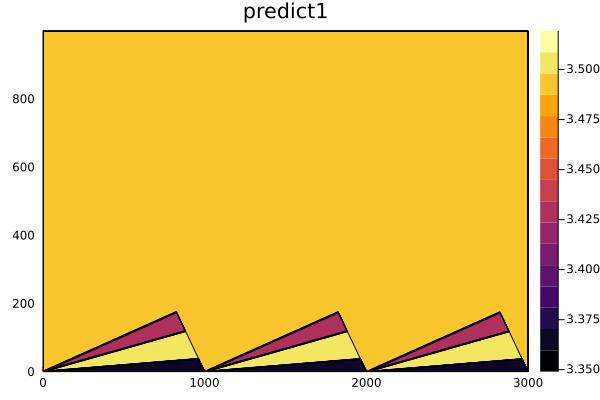
\includegraphics[width=0.45\linewidth]{sol_variable_corrected_bcs31.png}
  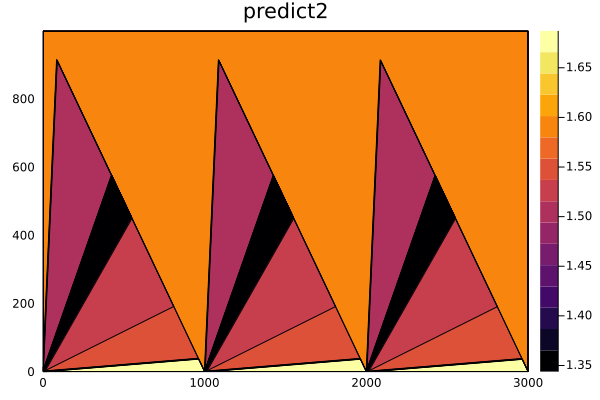
\includegraphics[width=0.45\linewidth]{sol_variable_corrected_bcs32.png}
  \\ %\legend{}
\end{figure}

Pretende-se, no entanto, utilizar das técnicas de discretização tradicionais, para o problema. Assim, por meio de Métodos das Diferenças Finitas, ou Elementos Finitos (MDF/MEF). Pois, são mais genéricas e seguras de se obter resultados desejados, como foi feito no artigo de Kerner (\autoref{fig:sim2}).

\begin{figure}[ht]
  \centering
  \caption{\label{fig:sim2} Simulação original. Fonte: Imagem de Kerner e Konhäuser \cite{kerner1993cluster}}
  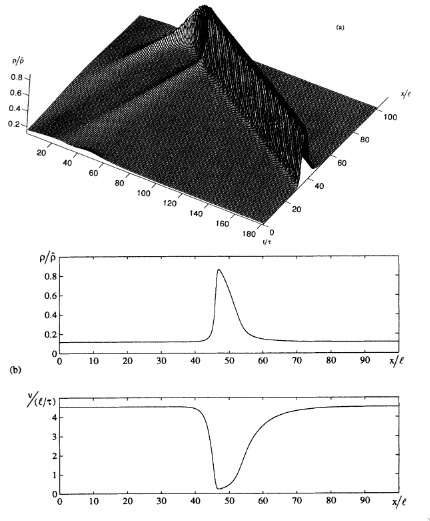
\includegraphics[width=0.4\linewidth]{kerner.png}
  \\  %\legend{Fonte: Imagem de Kerner e Konhäuser \cite{kerner1993cluster}}
\end{figure}


\clearpage
\bibliography{global-bib}
\bibliographystyle{acm}
\end{document}